\documentclass{article}
\usepackage[T2A]{fontenc}
\usepackage[utf8]{inputenc}
\usepackage{graphicx}
\usepackage[export]{adjustbox}
\usepackage{geometry}
\usepackage{float}
\usepackage{indentfirst}
% Preamble

% Packages
\usepackage{amsmath}

% Document
\begin{document}
    \begin{center}
    \hfill \break
    \large{МИНОБРНАУКИ РОССИИ}\\
    \footnotesize{ФЕДЕРАЛЬНОЕ ГОСУДАРСТВЕННОЕ БЮДЖЕТНОЕ ОБРАЗОВАТЕЛЬНОЕ УЧРЕЖДЕНИЕ}\\
    \footnotesize{ВЫСШЕГО ПРОФЕССИОНАЛЬНОГО ОБРАЗОВАНИЯ}\\
    \small{\textbf{«ВОРОНЕЖСКИЙ ГОСУДАРСТВЕННЫЙ УНИВЕРСИТЕТ»}}\\
    \hfill \break
    \normalsize{Факультет компьютерных наук}\\
    \hfill \break
    \normalsize{Кафедра программирования и информационных технологий}\\
    \hfill\break
    \hfill \break
    \hfill \break
    \hfill \break
    \large{Отчет по предмету Архитектура информационных систем
    \\1 лабораторная работа
    \\Приложение для автоматизированного проведения тестирования}\\
    \end{center}

    \hfill \break
    \hfill \break
    \hfill \break
    \hfill \break
    \hfill \break

    \begin{flushright} Вычиков Д.Д \end{flushright}
    \vspace*{\fill}
    \begin{center} Воронеж 2019 \end{center}
    \thispagestyle{empty}
    \newpage

    \section{Диаграммы IDEF0}
    \subsection{Контекстная диаграмма верхнего уровня}
    \begin{figure}[H]
        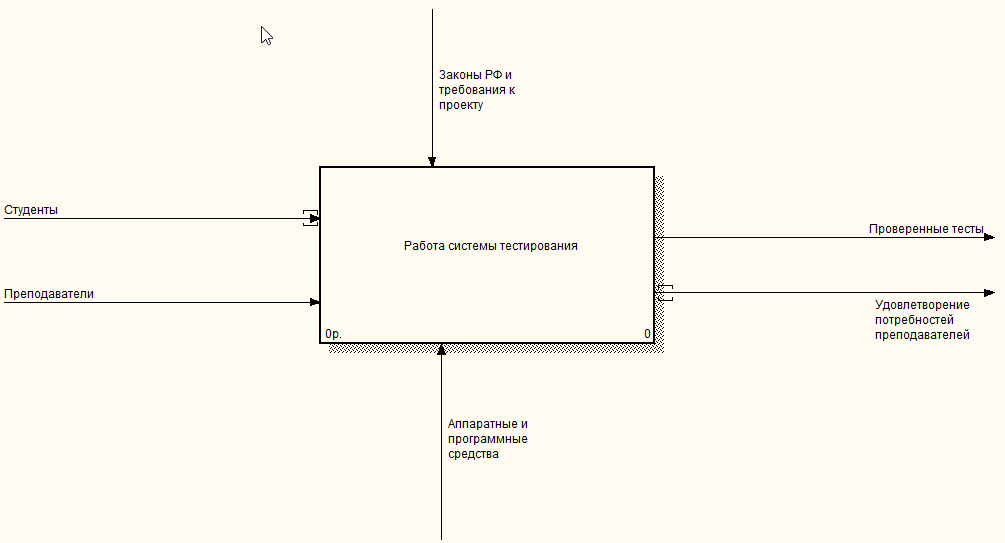
\includegraphics[width=\textwidth, center]{../img/idef0/idef0_context.png}
        \caption{Контекстная диаграмма верхнего уровня}
    \end{figure}

    Данная диаграмма является общим представлением работы автоматизированной
    системы для тестирования.

    На вход системы поступают преподаватели (администрароторы) и студенты
    (пользователи).

    Выходными блоками являются проверенные тестовые задания и удовлетворенные
    потребности преподавателей.

    Управление для данной системы осуществляют законы Российской Федерации,
    устанавливающие порядок обработки персональных данных, а также ряд других
    ограничений, и требования, предъявляемые к функциональности системы.

    Механизмами, выполняющими преобразования входных данных в выходные являются
    аппаратные и программные средства: компьютеры, операционная система,
    языки программирования, различные библиотеки и виртуальные среды для
    выполнения кода программы.

    \subsection{Работа системы тестирования}
    \begin{figure}[H]
        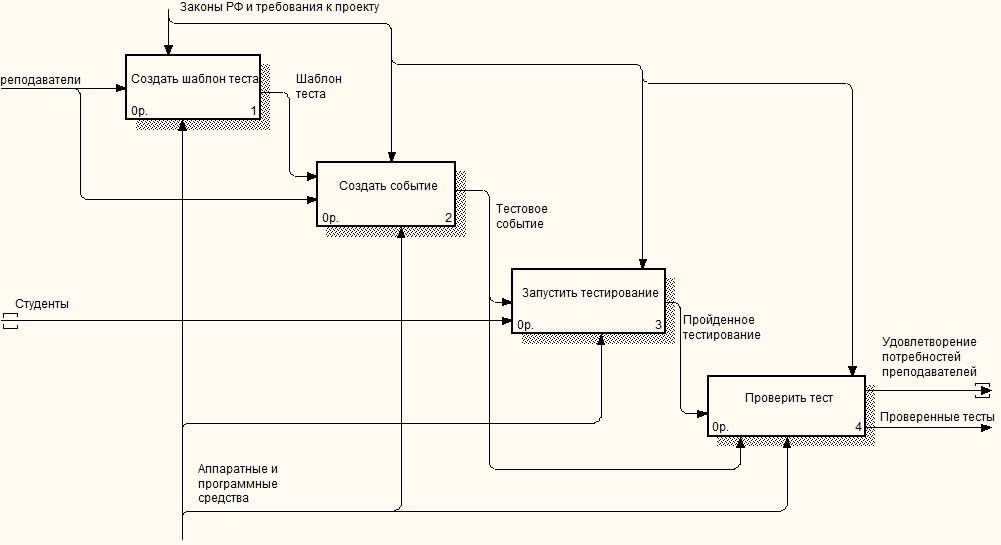
\includegraphics[width=\textwidth, center]{../img/idef0/context_decompose.png}
        \caption{Работа системы тестирования}
    \end{figure}

    Данная диаграмма раскрывает функциональный блок контекстной
    диаграммы верхнего уровня "Работа системы тестирования".

    Представленные функциональные блоки





\end{document}